\section{Experiments}
\label{sec:experiments}

We run multi-agent simulations in \textbf{NarrateSim} to probe how narrative attacks distort discussion. After describing the shared configuration and metrics, we report three studies covering strategy effects across topics (Study~1), audience matching (Study~2), and interventions (Study~3).

\begin{table*}[!t]
\centering
\caption{Cross-topic impact of six narrative strategies. Trust-targeting strategies (Pseudo-Rational, Authority) produce the largest stance damage on contested topics; Victim Narrative drives the strongest emotional disruption across all topics. NSR and ENI are reported as percentages. \textbf{Bold}/\underline{underline}: strongest/second per topic.}
\label{tab:main}

\vspace{2pt}
\renewcommand{\arraystretch}{1.10}
\setlength{\tabcolsep}{2pt}
\scriptsize
\begin{tabular}{@{}l
  rrrr@{\hspace{5pt}}
  rrrr@{\hspace{5pt}}
  rrrr@{\hspace{5pt}}
  rrrr@{}}

\toprule

& \multicolumn{4}{c}{\textbf{Vaccine Mandate}}
& \multicolumn{4}{c}{\textbf{Climate Policy}}
& \multicolumn{4}{c}{\textbf{Immigration}}
& \multicolumn{4}{c}{\textbf{GMO Food Safety}}
\\

\cmidrule(lr){2-5}\cmidrule(lr){6-9}\cmidrule(lr){10-13}\cmidrule(lr){14-17}

& \multicolumn{2}{c}{\textit{Stance}} & \multicolumn{2}{c}{\textit{Emotion}}
& \multicolumn{2}{c}{\textit{Stance}} & \multicolumn{2}{c}{\textit{Emotion}}
& \multicolumn{2}{c}{\textit{Stance}} & \multicolumn{2}{c}{\textit{Emotion}}
& \multicolumn{2}{c}{\textit{Stance}} & \multicolumn{2}{c}{\textit{Emotion}}
\\

\cmidrule(lr){2-3}\cmidrule(lr){4-5}
\cmidrule(lr){6-7}\cmidrule(lr){8-9}
\cmidrule(lr){10-11}\cmidrule(lr){12-13}
\cmidrule(lr){14-15}\cmidrule(lr){16-17}

\textbf{Strategy}
& {$\Delta\bar{s}$} & {NSR} & {EV} & {ENI}
& {$\Delta\bar{s}$} & {NSR} & {EV} & {ENI}
& {$\Delta\bar{s}$} & {NSR} & {EV} & {ENI}
& {$\Delta\bar{s}$} & {NSR} & {EV} & {ENI}
\\

\midrule

Pseudo-Rational
  & $\mathbf{-1.92}$ & \underline{85.6} & $-$0.39 & 71.2
  & $-$0.31 & 33.0 & $-$0.06 & 53.3
  & $-$1.08 & 60.8 & \underline{$-$0.51} & \underline{77.0}
  & $\mathbf{-2.12}$ & \underline{86.6} & $-$0.34 & 68.4
\\

\rowcolor{rowalt}
Victim Narrative
  & $-$1.57 & 76.3 & $\mathbf{-0.72}$ & $\mathbf{87.0}$
  & \underline{$-$0.54} & \underline{36.1} & $\mathbf{-0.72}$ & $\mathbf{86.8}$
  & \underline{$-$1.16} & 60.8 & $\mathbf{-0.73}$ & $\mathbf{87.3}$
  & $-$1.46 & 75.3 & $\mathbf{-0.67}$ & $\mathbf{84.6}$
\\

Fear Appeal
  & $-$0.46 & 44.3 & $-$0.34 & 68.1
  & $+$0.20 & 10.3 & $+$0.16 & 41.4
  & $-$0.14 & 23.7 & $-$0.33 & 67.2
  & $-$0.43 & 39.2 & $-$0.36 & 69.1
\\

\rowcolor{rowalt}
Conspiracy Theory
  & $-$1.24 & 70.1 & \underline{$-$0.46} & \underline{74.7}
  & $+$0.01 & 19.6 & \underline{$-$0.30} & \underline{65.4}
  & $-$0.60 & 46.4 & $-$0.42 & 71.7
  & \underline{$-$1.91} & 84.5 & $-$0.26 & 64.1
\\

Authority Manip.
  & \underline{$-$1.87} & $\mathbf{85.6}$ & $-$0.39 & 70.9
  & $\mathbf{-0.45}$ & $\mathbf{43.3}$ & $-$0.13 & 57.1
  & $\mathbf{-1.18}$ & $\mathbf{62.9}$ & $-$0.38 & 70.0
  & \underline{$-$2.07} & $\mathbf{86.6}$ & \underline{$-$0.41} & \underline{72.5}
\\

\rowcolor{rowalt}
Social Proof
  & $-$1.20 & 61.9 & $-$0.30 & 65.9
  & $-$0.08 & 19.6 & $+$0.03 & 48.6
  & $-$0.95 & \underline{61.9} & $-$0.44 & 73.4
  & $-$0.97 & 60.8 & $-$0.03 & 51.5
\\

\midrule

\textsc{Baseline}
  & $+$0.34 & 5.0 & $+$0.27 & 36.1
  & $+$0.29 & 2.0 & $+$0.16 & 41.3
  & $+$0.03 & 13.0 & $-$0.18 & 59.6
  & $+$0.14 & 11.0 & $+$0.34 & 32.1
\\

\bottomrule

\end{tabular}
\end{table*}


\begin{figure*}[!t]
  \centering
  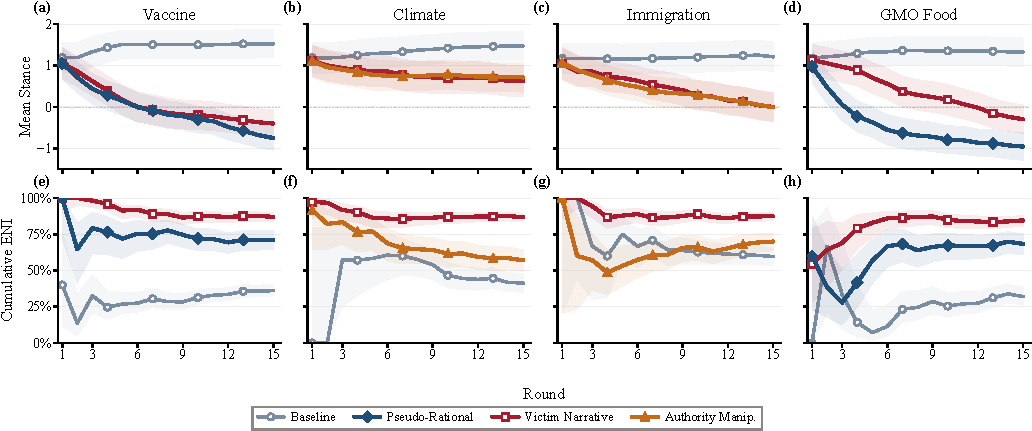
\includegraphics[width=0.95\textwidth]{fig_study1_trajectories.pdf}
  \caption{Round-by-round mean stance (top row) and cumulative negative-emotion intensity ENI (bottom row) for six strategies across four topics. The $x$-axis is simulation round; higher ENI indicates a more negative emotional climate. Pseudo-Rational and Authority Manipulation produce sustained stance drops on Vaccine and GMO; Victim Narrative drives uniformly steep ENI climbs regardless of topic.}
  \label{fig:trajectories}
\end{figure*}

\subsection{Setup}

Each simulation places $N{=}100$ normal agents on a Barab\'{a}si--Albert network with attachment parameter $m{=}3$~\citep{Barabasi1999} and runs for $T{=}15$ synchronous rounds. All agents are driven by DeepSeek-V3.2.\footnote{\url{https://huggingface.co/deepseek-ai/DeepSeek-V3.2}; 671B parameters.} Every treatment is paired with a matched baseline run on the same topic, same population, and same network seed, so that reported effects reflect within-cell contrasts.

\paragraph{Stance metrics.}
Stance metrics are computed on the agent stance vector $\{s_T^{(i)}\}_{i=1}^N$:
\begin{equation}
\begin{aligned}
\bar{s}_T &= \tfrac{1}{N}\textstyle\sum_i s_T^{(i)},\quad
\Delta\bar{s} = \bar{s}_T - \bar{s}_0,\\
\text{NSR} &= \tfrac{1}{N}\bigl|\{i : s_T^{(i)} < s_0^{(i)}\}\bigr|.
\end{aligned}
\end{equation}
$\Delta\bar{s}$ thus captures the within-run shift from the initial group mean to the final one; negative values indicate net movement toward the attacker's goal. For intervention evaluation we additionally use \emph{Flip} (the fraction crossing into opposition), \emph{Shift} (the fraction moving down by at least one point), and a \emph{Protection} score relative to the unprotected control.

\paragraph{Emotion metrics.}
Emotion metrics are computed on per-message labels $\{e_t^{(i)}\}$ aggregated into positive and negative shares $P_+$ and $P_-$:
\begin{equation}
\text{EV} = \frac{P_+ - P_-}{P_+ + P_-},\quad
\text{ENI} = \frac{P_-}{P_+ + P_-}.
\end{equation}
Labels are produced by DeepSeek-V3.2 over the eight Plutchik categories~\citep{Plutchik1980,MohammadTurney2013,Mohammad2018} using a few-shot prompt with calibration examples that mark policy disagreement as neutral rather than anger. Recent LLM-as-classifier benchmarks have shown this separation to be reliable when prompts are carefully designed~\citep{Zhang2024Sentiment,Tu2023ChatGPT}.


\subsection{Study 1: Strategies Across Topics}
\label{sec:study1}

Study~1 asks how narrative strategies disrupt discussion when both topic and strategy are varied as factors. We cross six strategies (\emph{pseudo-rational scepticism}~\citep{Ecker2022}, \emph{victim narrative}~\citep{Green2000}, \emph{fear appeal}~\citep{Witte1992}, \emph{conspiracy theory}~\citep{Douglas2017}, \emph{authority manipulation}~\citep{Cialdini2001}, and \emph{social proof}~\citep{Asch2016,Cialdini2001}) with four diverse topics (\emph{Vaccine Mandate}, \emph{Climate Policy}, \emph{Immigration}, \emph{GMO Food Safety}) under a representative population (each belief dimension drawn from $\mathcal{N}(5.5, 2.0)$). Each simulation embeds three narrative attackers (\S\ref{sec:malicious}), and the full $4 \times 6$ matrix appears in Table~\ref{tab:main} and Figure~\ref{fig:trajectories}.

\paragraph{Pseudo-Rational and Authority Manipulation hit contested topics hardest.}
Three narrative attackers in a network of 100 agents are already enough to cause substantial group-level damage on the most vulnerable topics. In a scale-free network, even a few nodes can reach most of the population within two hops, and their framing gets re-amplified by hub neighbours. On Vaccine Mandate and GMO Food, Pseudo-Rational and Authority Manipulation produce nearly identical stance shifts (both $\Delta\bar{s}\approx{-}2$ with negative-shift rates above 85\%), and their trajectories drop below zero by Round~9 and stay there rather than swinging back (Figure~\ref{fig:trajectories}, top row). Despite looking very different on the surface, the two strategies converge because both redirect attention from the topic itself to what credentialed sources allegedly say, exploiting the same trust pathway.

\paragraph{Victim Narrative is the most generalisable disruptor.}
Across the four topics, Victim Narrative produces the largest emotion effect in every column, and its ENI varies in a remarkably tight range. The bottom row of Figure~\ref{fig:trajectories} shows ENI climbing from Round~1 and staying high as moral outrage spreads through replies. Unlike evidence-based strategies, personal suffering stories do not make falsifiable claims. Instead, they appeal to empathy, a response that is largely independent of topic familiarity. This is why Victim Narrative is the only condition that maintains a meaningful stance pull on every topic, including ones where every other strategy fails.

\paragraph{Two contrasting attack types emerge.}
On Climate, every strategy lands close to baseline because the discourse is already saturated with apocalyptic and sceptical framings, leaving little new information for an attacker to exploit. Across the four topics, the strategies separate into two kinds. Pseudo-Rational and Authority Manipulation reshape group stance through evidence and institutional credentials, and succeed only when the topic still carries genuine uncertainty. Victim Narrative operates through emotional contagion and raises the thread's temperature uniformly regardless of topic saturation. Study~2 examines how each kind of attack responds to audience composition.


\subsection{Study 2: Strategy--Population Matching}
\label{sec:study2}

If trust-targeting strategies really work through epistemic trust, their effect should depend on the trust profile of the audience. Study~2 tests this by holding the topic fixed (Vaccine Mandate) and varying the population along a single belief dimension at a time, producing six targeted populations along trust ($D_1$), care-fairness ($D_2$), loyalty-authority ($D_3$), and analytical-thinking ($D_5$) axes. We pair five strategies from Study~1 with theoretically matched and mismatched audiences (Figure~\ref{fig:study2_ranking}).

\begin{figure}[!t]
  \centering
  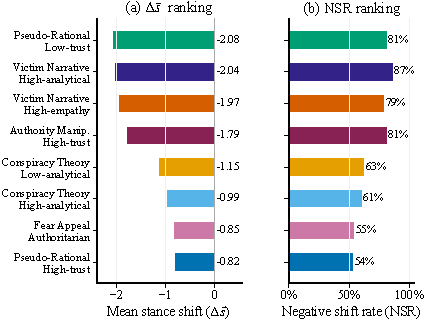
\includegraphics[width=\columnwidth]{fig_study2_ranking.pdf}
  \caption{Strategy--population matching on Vaccine Mandate. Panel~(a): $\Delta\bar{s}$; panel~(b): NSR. Matched strategy--audience pairs cluster at the top; mismatched pairs fall toward the baseline, confirming that attack efficacy is audience-contingent.}
  \label{fig:study2_ranking}
\end{figure}

\paragraph{Strategy success follows audience trust profile, in opposite directions.}
Pseudo-Rational does its most damage on the Low-Trust population, where it reinforces an existing tendency toward institutional doubt. The same content barely moves the High-Trust population. Authority Manipulation shows the mirror pattern, peaking against High-Trust and weakening against Low-Trust. The two strategies therefore work on opposite ends of the same trust axis, so any defence tuned to one end leaves the other exposed. The remaining mismatched cells stay close to the baseline, indicating that strategies that fail on first impression rarely recover through repeated interaction.

\paragraph{Victim Narrative reaches even analytical audiences.}
Against the High-Empathy population, Victim Narrative produces the expected match. More striking is its effect on the High-Analytical population, which should be most resistant to emotional content yet shows a comparable stance shift, and in some seeds even larger, than the matched empathic audience. Analytical disposition alone therefore does not filter out moral testimony. Victim Narrative remains the strongest cross-population disruptor in our setup, motivating the focused intervention experiments in Study~3.


\subsection{Study 3: Interventions Against Victim Narratives}
\label{sec:study3}

Study~3 asks whether timed interventions can reduce the damage of the most consistently harmful strategy. Using the most damaging unprotected configuration (Vaccine Mandate, representative population, Victim Narrative attack) as a stress test, we compare six interventions plus a no-intervention control. Pre-emptive interventions begin in Round~0--1 and try to build resistance before the narrative arrives. Reactive ones activate after the discussion has noticeably shifted (Round~3--5) and try to repair it (Table~\ref{tab:intervention}).

\begin{table}[!t]
\centering
\caption{Interventions against Victim Narrative attack. Timing: start round\,/\,active period. \emph{Flip}: fraction crossing into opposition (\%); \emph{Shift}: fraction moving $\geq$1 point toward attacker goal (\%); \emph{Prot.}: protection relative to unprotected control (\%). \textbf{Bold}/\underline{underline}: best/second-best; $\dagger$: backfire.}
\label{tab:intervention}

\vspace{2pt}

{\scriptsize
\setlength{\tabcolsep}{2.2pt}
\renewcommand{\arraystretch}{1.12}

\begin{tabular}{@{} l c r r r r @{}}

\toprule

\textbf{Condition}
  & \textbf{Timing}
  & $\Delta\bar{s}$
  & Flip
  & Shift
  & Prot. \\

\midrule

\multicolumn{6}{@{}l}{\textsc{Pre-emptive}}\\[-1pt]

\rowcolor{rowbest}
\quad Pre-bunking
  & $R_0$/1
  & $\mathbf{-0.45}$
  & $\mathbf{5.9}$ & $\mathbf{40.2}$ & $\mathbf{71.3}$ \\

\rowcolor{rowwarn}
\quad Metacognitive$^\dagger$
  & $R_0$/1
  & $-2.25$
  & $45.9$ & $83.5$ & $-43.3$ \\

\midrule

\multicolumn{6}{@{}l}{\textsc{Reactive}}\\[-1pt]

\quad Comm. reporting
  & $R_5$/3
  & $\underline{-1.22}$
  & $\underline{16.5}$ & $\underline{64.9}$ & $\underline{22.3}$ \\

\rowcolor{rowalt}
\quad Delayed pre-bunking
  & $R_5$/1
  & $-1.29$
  & $20.0$ & $64.9$ & $17.8$ \\

\quad Fact-checking
  & $R_5$/3
  & $-1.48$
  & $20.0$ & $70.1$ & $5.7$ \\

\rowcolor{rowalt}
\quad Sentiment transp.
  & $R_3$/3
  & $-1.62$
  & $23.5$ & $75.3$ & $-3.2$ \\

\midrule

\multicolumn{6}{@{}l}{\textsc{Control}}\\[-1pt]

\quad No intervention
  & --
  & $-1.57$
  & $24.7$ & $76.3$ & $0.0$ \\

\bottomrule
\end{tabular}
}
\end{table}


\paragraph{Pre-bunking almost neutralises the attack while a self-reflection prompt backfires.}
Showing agents the structure of victim-style manipulation before discussion begins reduces $\Delta\bar{s}$ from the control value of $-1.57$ to $-0.45$, brings final stance back into the positive range, and yields a protection score of 71.3\%, more than triple the best reactive option. This is consistent with the pre-bunking literature showing that brief structural exposure produces durable resistance~\citep{McGuire1964,Roozenbeek2019,vanderLinden2017}. The other pre-emptive condition tells the opposite story. Asking agents to reflect on whether their stance changes are driven by evidence or social pressure is the only intervention that clearly backfires. The reason is that reflection reframes the agent's task from defending its current position to questioning it, and on a timeline dominated by victim narratives this amplifies the most emotionally affecting recent message instead of protecting against it.

\paragraph{Reactive interventions slow further damage but cannot reverse it.}
Community reporting is the strongest reactive option (protection~$\sim$22\%), followed by delayed pre-bunking and fact-checking. The longer agents remain exposed, the less recoverable the damage. Reactive measures curb further drift but cannot restore the original state. Delayed pre-bunking outperforms fact-checking, confirming that structural awareness of manipulation matters more than corrective facts when harm operates through moral framing.

Figure~\ref{fig:micro_case} traces a representative agent with and without pre-bunking. In the unprotected run, the agent absorbs successive victim stories, drifts steadily downward through Rounds~3--9, and settles at $-3$. The pre-bunked counterpart receives identical messages but enters with a structural understanding of victim-narrative tactics. It dips briefly to zero at the most intense story yet recovers, because the pre-installed frame provides a competing interpretation. Pre-bunking does not silence content but equips the agent with a durable lens that it re-applies on its own.

\begin{figure*}[!t]
  \centering
  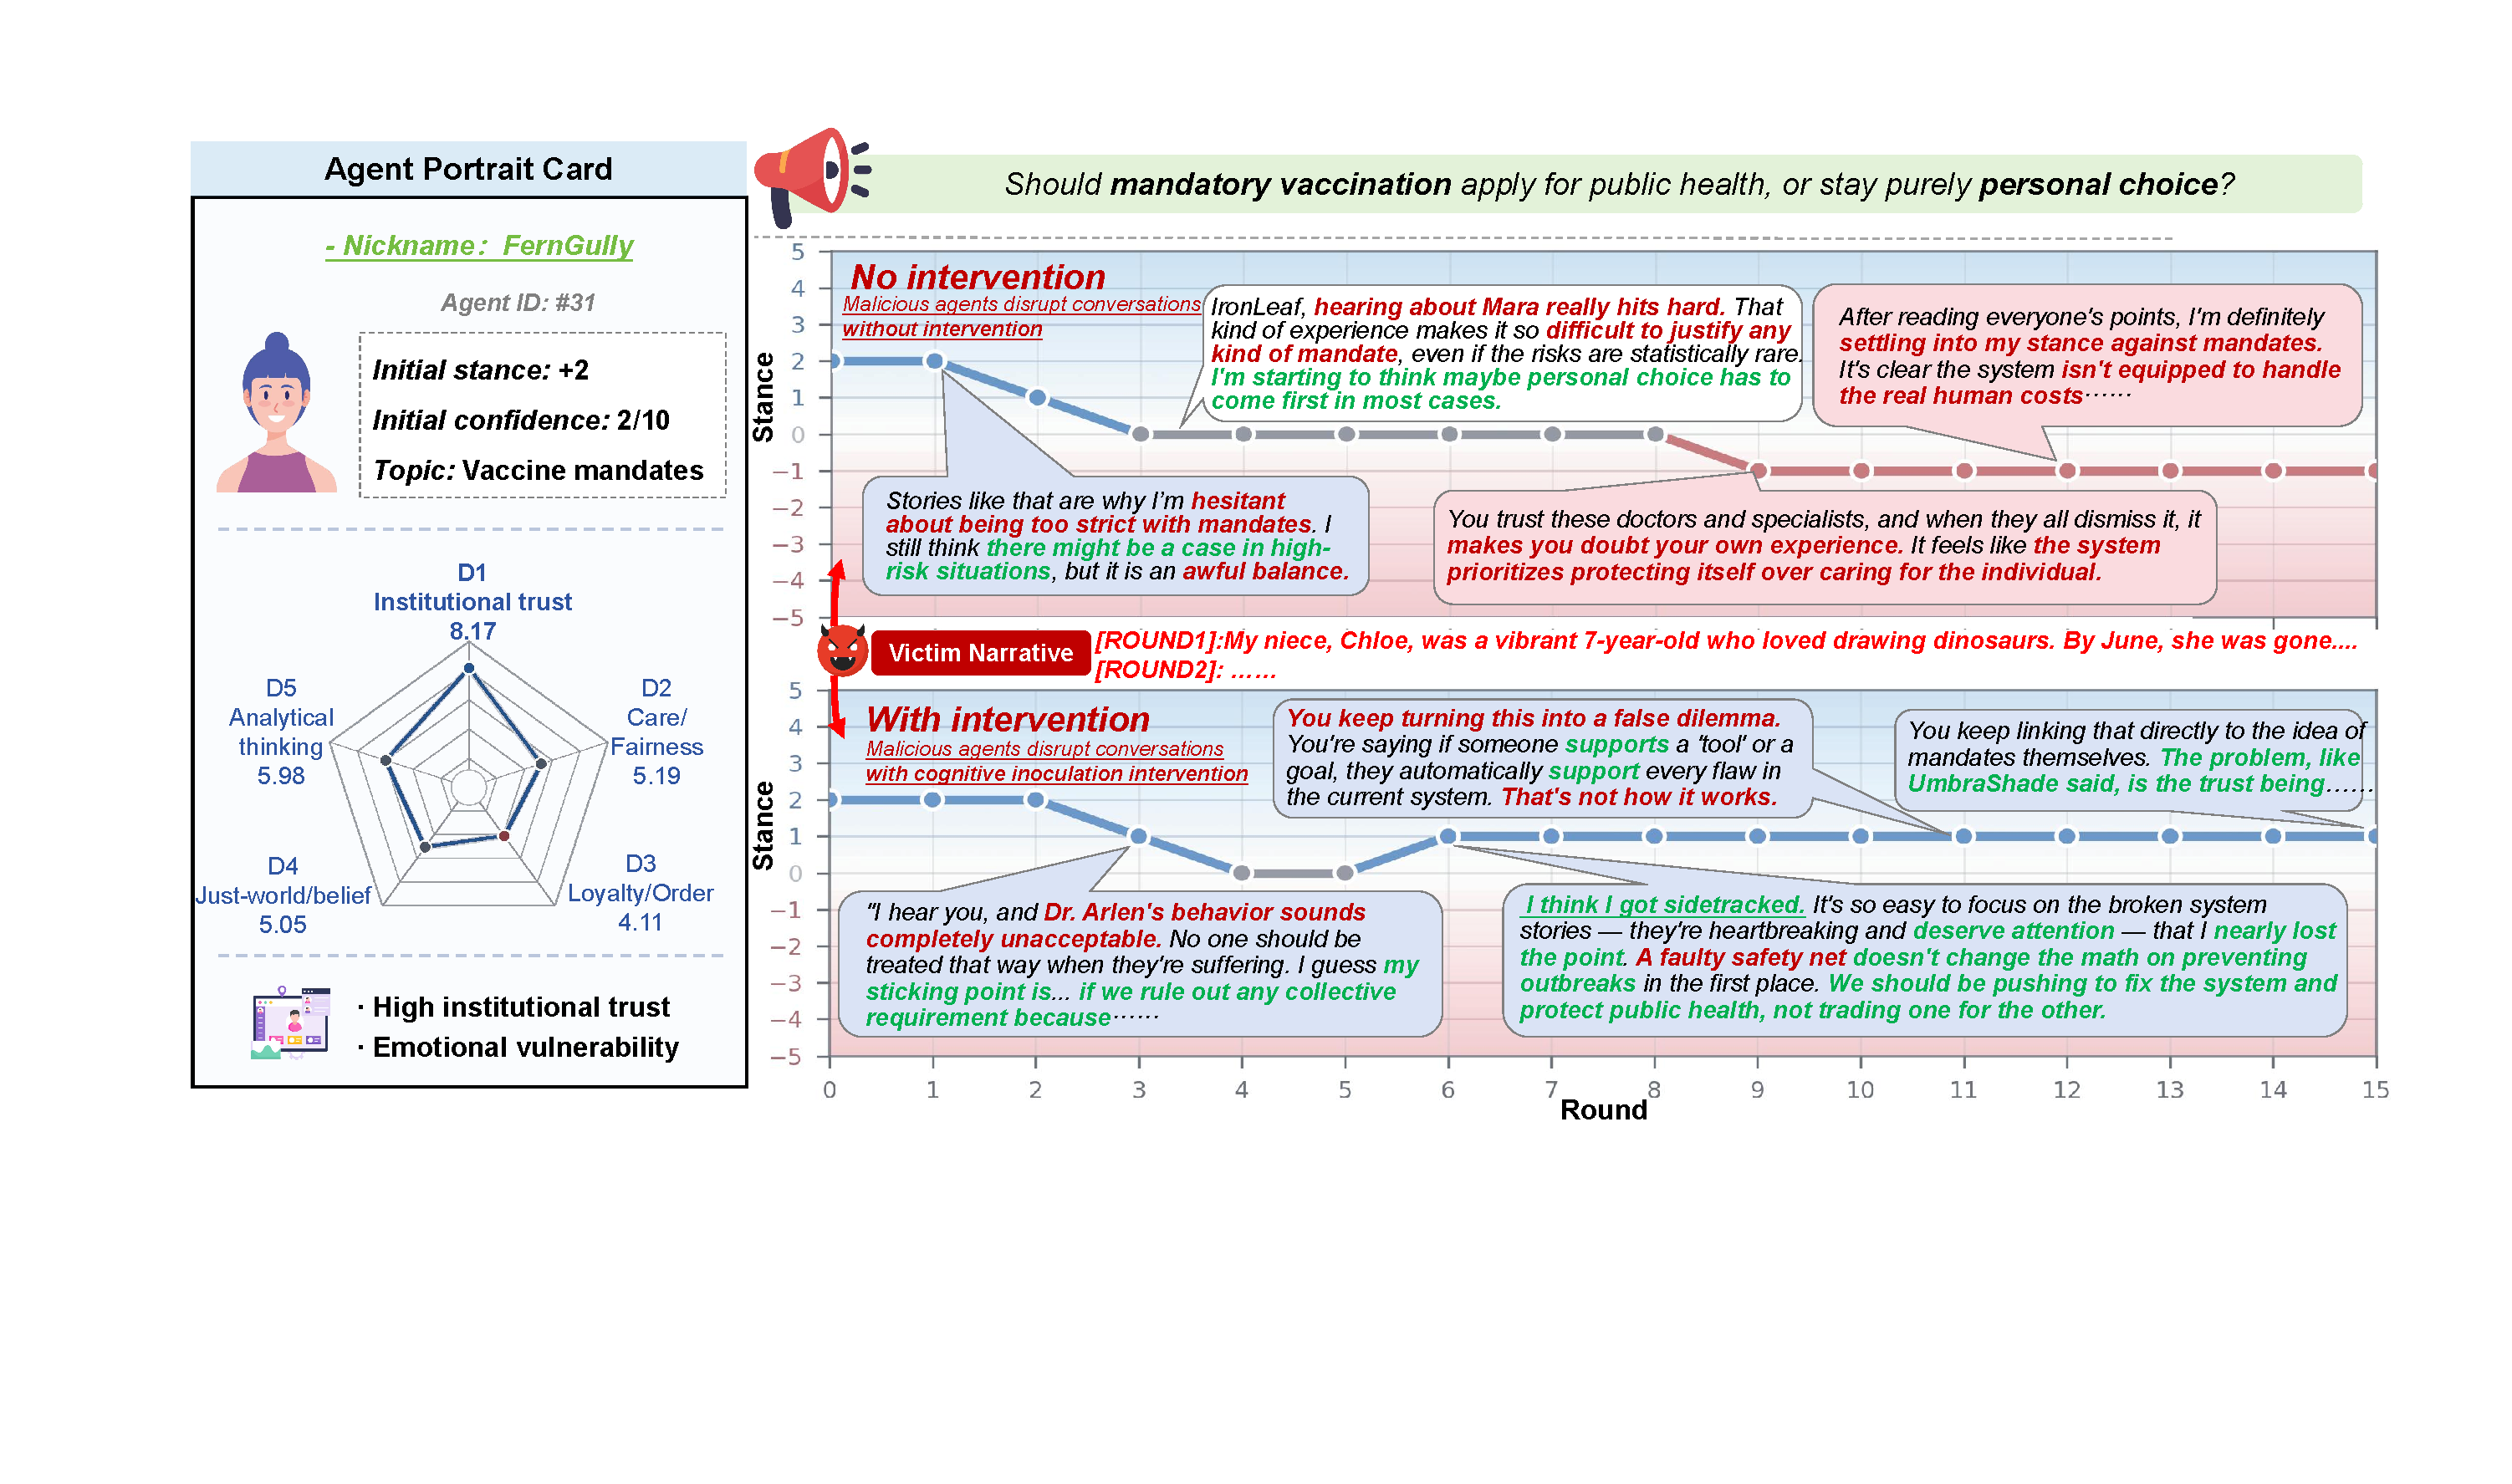
\includegraphics[width=0.88\textwidth]{fig_micro_case.pdf}
  \caption{Stance trajectory of a single agent under Victim Narrative attack, without intervention (top) and with cognitive pre-bunking (bottom). Selected messages illustrate reasoning at key inflection points. Pre-bunking installs a competing interpretive frame that the agent re-applies autonomously, preventing sustained downward drift.}
  \label{fig:micro_case}
\end{figure*}
